% acl.tex — main draft (ACL anthology format)
% Requires: acl.sty from https://github.com/acl-org/acl-style-files
% Build: pdflatex acl && bibtex acl && pdflatex acl && pdflatex acl

\documentclass[11pt]{article}

% Switch to \usepackage[review]{acl} when acl.sty is installed
\usepackage[margin=1in]{geometry}
\usepackage{times}
\usepackage{latexsym}
\usepackage{amsmath,amssymb}
\usepackage{graphicx}
\usepackage{booktabs}
\usepackage{hyperref}
\usepackage{natbib}

\title{Can Unsupervised Pre-Inference Signals Support Appropriate Multi-LLM Routing?}

\author{
  Anonymous Author(s) \\
  Anonymous Institution \\
  \texttt{anonymous@domain.edu}
}

\begin{document}
\maketitle

\begin{abstract}
Multi-LLM systems must select an appropriate model per query while trading off quality and cost, yet most work develops routing algorithms using supervised labels or post-generation information \citep{ong2024routellm,guha2024smoothie}.
We ask: \textbf{can unsupervised pre-inference signals support appropriate multi-LLM routing before generation?}
We organize unsupervised pre-inference signals as \textbf{latent routing dimensions} with prefill operationalizations, ask which dimensions predict routing opportunity, and evaluate whether a calibrated logistic policy can exploit them on a held-out test split.
On ARC-Challenge ($n{=}299$ calibration, $n{=}1{,}172$ test; Llama~3.2~1B/3B): \textbf{(1)}~multiple \textbf{latent routing dimensions} predict opportunity before generation (best operationalization: AUROC ${\sim}0.61$ for escalation potential); \textbf{(2)}~dimensions encode different routing need---task difficulty and model uncertainty overlap, while model disagreement and escalation potential separate routable from irrecoverable hard queries; \textbf{(3)}~a CALIB-fit calibrated policy matches always routing to the strong model (69.2\% vs.\ oracle 74.4\%), leaving 5.2 percentage points unexploited.
Signal extraction is unsupervised at inference time; oracle labels supply characterization evidence; the routing policy uses supervised calibration on CALIB for evaluation only.
\end{abstract}

% §1 Introduction

\section{Introduction}
\label{sec:intro}

Large language models (LLMs) vary widely in capability and inference cost.
Deploying a single model for every query is inefficient: some inputs are answered correctly by a small model, while others require a larger one \citep{hu2024routerbench,ding2024hybrid,chen2023frugalgpt}.
\textbf{Multi-LLM routing} assigns each query to a model in a fixed pool $\mathcal{M}$ so as to trade off response quality against inference cost \citep{ong2024routellm}.

\paragraph{Problem.}
The routing objective is \textbf{appropriate model selection}: route to the \textbf{weakest model expected to answer correctly}, escalating only when additional capability is likely to help.
Most prior work develops \textbf{routing algorithms}---supervised routers \citep{ong2024routellm,ding2024hybrid,feng2025graphrouter}, learned pre-hoc estimators \citep{cao2026scope}, or post-generation selectors \citep{guha2024smoothie,niu2026cascal}.
We instead ask a prior question: \textbf{what routing-relevant information is available before any routing decision is made?}
Specifically, can \textbf{unsupervised pre-inference signals}---statistics derived from query text and prefill probes before full generation---support appropriate model selection?

\paragraph{Research question.}
\textit{Can unsupervised pre-inference signals support selecting the appropriate LLM from a fixed pool before generation?}

We do not ask which isolated statistic achieves the highest AUROC.
We ask which \textbf{latent routing dimensions}---task difficulty, model uncertainty, model disagreement, escalation potential---are measurable before generation, and whether a calibrated policy can use them (Table~\ref{tab:dimensions}).

\paragraph{Approach.}
We treat routing need as \textbf{latent}: each dimension is \textbf{operationalized} by one prefill statistic (e.g., task difficulty by \texttt{piece\_count}; escalation potential by $\Delta m_{\mathrm{gain}}$).
Studies I--III ask \textbf{which dimension predicts routing opportunity} and whether dimensions encode \textbf{different} aspects of that need.
Signal characterization supplies \textbf{evidence}; routing evaluation supplies \textbf{validation} (\S\ref{sec:routing}).

\paragraph{What ``unsupervised'' means.}
\textbf{Signal extraction} is unsupervised at inference time.
Offline oracle labels evaluate whether each dimension predicts opportunity (Studies I--III).
Routing evaluation fits a demonstration policy on CALIB only (\S\ref{sec:method:supervision}).

\paragraph{Contributions.}
\begin{enumerate}
  \item An empirical study of \textbf{unsupervised pre-inference signals} for multi-LLM routing, with appropriate selection defined over a fixed pool and no routing labels at extraction time.
  \item A dimensional account of routing need: four \textbf{latent routing dimensions} with prefill operationalizations (Table~\ref{tab:dimensions}).
  \item \textbf{Empirical evidence} on ARC-Challenge: multiple dimensions predict opportunity; \textbf{task difficulty and model uncertainty} overlap, while \textbf{model disagreement and escalation potential} separate routable from irrecoverable hard queries; dimensions are partially complementary (\S\ref{sec:characterization}).
  \item \textbf{Routing evaluation}: a calibrated logistic policy leaves exploitable headroom relative to an offline oracle (\S\ref{sec:routing}).
\end{enumerate}

\paragraph{Main findings (ARC test, $n{=}1{,}172$).}
The answer is \textbf{partially}.
\begin{enumerate}
  \item \textbf{Dimensions predict opportunity.} Routing opportunity occurs on 43.3\% of queries; escalation potential reaches AUROC ${\sim}0.61$ (Table~\ref{tab:study2}).
  \item \textbf{Dimensions differ.} Model uncertainty does not separate opportunity from too-hard queries ($d{\approx}0.03$); escalation potential does ($d{\approx}0.72$).
  \item \textbf{Routing leaves headroom.} A CALIB-fit calibrated policy matches always-strong (69.2\%); oracle 74.4\% (Table~\ref{tab:routing}).
\end{enumerate}

\paragraph{Paper organization.}
\S\ref{sec:related}--\S\ref{sec:setup} set context and methodology.
\S\ref{sec:characterization} tests which dimensions predict opportunity.
\S\ref{sec:routing} reports routing evaluation.


% §2 Related Work

\section{Related Work}
\label{sec:related}

Prior routing work primarily \textbf{develops routing algorithms}.
We instead ask what \textbf{routing-relevant information is available before any routing decision}---when it becomes available, what unsupervised pre-inference signals encode, and whether that information supports appropriate model selection.
Table~\ref{tab:landscape} organizes work by timing; we situate our study in the \textbf{before inference} column.

\begin{table}[t]
  \centering
  \small
  \begin{tabular}{p{0.20\linewidth}p{0.32\linewidth}p{0.36\linewidth}}
    \toprule
    \textbf{When} & \textbf{Typical routing inputs} & \textbf{Representative work} \\
    \midrule
    Before inference &
      Query text; prefill logits; anchor fingerprints &
      CP-Router, SCOPE, \textbf{this work} \\
    During inference &
      Query embeddings; preference classifiers; graph histories &
      RouteLLM, Hybrid LLM, GraphRouter \\
    After generation &
      Full responses; output embeddings; cascades &
      Smoothie, CASCAL, FrugalGPT, Mu et al. \\
    Evaluation only &
      Precomputed outcomes &
      RouterBench \\
    \bottomrule
  \end{tabular}
  \caption{Related work by when routing information becomes available.}
  \label{tab:landscape}
\end{table}

\paragraph{Before inference.}
SCOPE trains a reasoning estimator on anchor-set correctness and cost \citep{cao2026scope}---a routing \emph{system}, not a study of what unsupervised prefill probes encode.
CP-Router uses conformal-prediction set size from MCQ logits for a binary LLM$\leftrightarrow$LRM choice \citep{su2025cprouter}.
\textbf{Our work} studies unsupervised pre-inference signals for multi-LLM routing: extract signals before generation, test which \textbf{latent routing dimensions} predict opportunity, and evaluate whether a calibrated policy can exploit them.

\paragraph{During inference (query-centric routers).}
RouteLLM learns $P(\text{strong wins} \mid q)$ from preference data without live per-model prefill probes \citep{ong2024routellm}.
Hybrid LLM trains a DeBERTa encoder on offline quality proxies \citep{ding2024hybrid}.
GraphRouter learns over query--LLM edges with historical performance \citep{feng2025graphrouter}.
These reduce cost but rely on supervised labels; they do not quantify unsupervised per-model prefill information.

\paragraph{After generation.}
Smoothie, CASCAL, FrugalGPT, and Mu et al.\ require full pool responses (or retrievals) before selection \citep{guha2024smoothie,niu2026cascal,chen2023frugalgpt,mu2025ragrouting}.
We study whether cheaper prefill probes suffice.

\paragraph{Logits, uncertainty, and evaluation.}
Logits may rank routing need despite miscalibration \citep{he2023uncertainty,plaut2024chat,kadavath2022language}.
RouterBench compares router families on precomputed outcomes \citep{hu2024routerbench} but does not study unsupervised prefill probes or how \textbf{latent routing dimensions}---task difficulty and model uncertainty versus model disagreement and escalation potential---structure routing need.

\paragraph{Positioning.}
We do not propose another supervised router or post-generation selector.
We investigate whether \textbf{routing-relevant information before generation} can support appropriate multi-LLM routing, with honest routing evaluation---including negative exploitation results \citep{plaut2024chat,hu2024routerbench}.


% §3 Method

\section{Method}
\label{sec:method}

We formalize unsupervised pre-inference routing (\S\ref{sec:method:formulation}), define \textbf{latent routing dimensions} and their operationalizations (\S\ref{sec:method:dimensions}), describe prefill-based signal extraction (\S\ref{sec:method:extraction}), and define evaluation metrics.
Experimental configuration: \S\ref{sec:setup}; empirical evidence: \S\ref{sec:characterization}; routing evaluation: \S\ref{sec:routing}.

\subsection{Routing formulation}
\label{sec:method:formulation}

Let $\mathcal{M}=\{M_1,\ldots,M_k\}$ be a fixed pool with known cost tiers \citep{hu2024routerbench,ding2024hybrid}.
For each query $q$, routing assigns one $M_i \in \mathcal{M}$ with objective \textbf{appropriate model selection}: route to the \textbf{weakest model expected to answer correctly}.

\textbf{Unsupervised pre-inference routing} uses query text and prefill probes before full generation, without routing supervision at extraction time \citep{guha2024smoothie,mu2025ragrouting}.
Prior work often ranks isolated statistics (e.g., entropy vs.\ margin).
We instead ask which \textbf{latent routing dimensions}---unobserved aspects of routing need---are measurable before generation and whether they predict \textbf{routing opportunity}.

\paragraph{Research hypotheses.}
\begin{align*}
  \text{RH1:}& \;\text{latent routing dimensions carry measurable predictive content for routing opportunity} \\
  \text{RH2:}& \;\text{dimensions encode different aspects of routing need} \\
  \text{RH3:}& \;\text{dimensions provide complementary predictive content beyond any single dimension} \\
  \text{RH4:}& \;\text{a calibrated routing policy can exploit available information.}
\end{align*}

\paragraph{Routing need (evaluation).}
For $(M_w,M_s)$, \textbf{routing opportunity} is $y(q,M_w)=0$ and $y(q,M_s)=1$ ($y^{\text{opp}}$).
Offline oracle labels $y(q,M_i)$ come from full greedy inference (\S\ref{sec:method:extraction}); they never enter signal extraction.
Four buckets---easy, opportunity, weak-only, too-hard---structure dimension-wise characterization.

\subsection{Latent routing dimensions}
\label{sec:method:dimensions}

A \textbf{latent routing dimension} is an aspect of routing need that is not observed directly---for example, how difficult the task is for the pool, how uncertain the weak model is, or whether escalation to the strong model is likely to help.
Each dimension is \textbf{operationalized} by a deterministic statistic computed from query text or prefill logits (Table~\ref{tab:dimensions}).

\paragraph{Scientific unit.}
The unit of analysis is the \textbf{dimension}, not the statistic.
Entropy, \texttt{piece\_count}, and $\Delta m_{\mathrm{gain}}$ are \emph{operationalizations}; the research question is whether the underlying dimension predicts opportunity.
Studies I--II therefore ask, for each dimension: \textbf{does this aspect of routing need predict $y^{\text{opp}}$?}
We report $\rho$ and AUROC as summaries of detectability---not as a feature leaderboard.

% Latent routing dimensions and their operationalizations (main analysis).
\begin{table}[t]
  \centering
  \small
  \setlength{\tabcolsep}{5pt}
  \begin{tabular}{@{}llp{0.42\linewidth}@{}}
    \toprule
    \textbf{Latent routing dimension} & \textbf{Operationalization} & \textbf{Measurement source} \\
    \midrule
    \textbf{Task difficulty} &
    $c(q)=$ \texttt{piece\_count} &
    Query text (model-independent) \\
    \addlinespace
    \textbf{Model uncertainty} &
    $H_w$ &
    Weak-model prefill logits \\
    \addlinespace
    \textbf{Model disagreement} &
    $\Delta H = H_w - H_s$ &
    Paired weak/strong logits \\
    \addlinespace
    \textbf{Escalation potential} &
    $\Delta m_{\mathrm{gain}} = m_s - m_w$ &
    Paired weak/strong logits \\
    \bottomrule
  \end{tabular}
  \caption{Latent routing dimensions and operationalizations studied in the main analysis. Dimensions are \emph{not} observed directly; each is measured through one CALIB-selected statistic. Appendix audits alternate operationalizations (e.g., $m_w$ for model uncertainty; Table~\ref{tab:md-variants}).}
  \label{tab:dimensions}
\end{table}


\paragraph{Operationalization details.}
\textbf{Task difficulty} is measured by $c(q)=$ \texttt{piece\_count}, selected on CALIB from query-text candidates (appendix Table~\ref{tab:d46}).
\textbf{Model uncertainty} uses weak-model entropy $H_w$ at the final prefill position \citep{he2023uncertainty,plaut2024chat}.
\textbf{Model disagreement} and \textbf{escalation potential} use paired weak/strong logits: $\Delta H = H_w - H_s$ and $\Delta m_{\mathrm{gain}} = m_s - m_w$.
Appendix Table~\ref{tab:md-variants} audits alternate operationalizations (e.g., $m_w$ as an alternative to $H_w$ for model uncertainty).

\subsection{Prefill-based signal extraction}
\label{sec:method:extraction}

Table~\ref{tab:pipeline} summarizes the analytical pipeline.
\textbf{Signal extraction} performs one prefill forward pass per pool member.
Richer measurements (trajectories, hidden states) would change operationalizations but not the dimensional abstraction.

% Analytical pipeline (orthogonal to dimension taxonomy in Table~\ref{tab:dimensions}).
\begin{table}[t]
  \centering
  \small
  \begin{tabular}{@{}clp{0.58\linewidth}@{}}
    \toprule
    & \textbf{Stage} & \textbf{Description} \\
    \midrule
    1 & Signal extraction &
    Query text; prefill logits at $t{=}T$ per pool member \\
    2 & Statistic computation (offline) &
    One representative per studied dimension (Table~\ref{tab:dimensions}) \\
    3 & Signal characterization &
    Routing-relevant information; cross-dimension structure; complementarity \\
    4 & Routing evaluation &
    Calibrated logistic policy; offline oracle; exploitation gap \\
    \bottomrule
  \end{tabular}
  \caption{Analytical pipeline. Each stage tests \textbf{latent routing dimensions} operationalized by prefill statistics---not isolated feature rankings.}
  \label{tab:pipeline}
\end{table}


\paragraph{Statistic definitions.}
\label{sec:method:prefill}
Task difficulty: $c(q)=$ \texttt{piece\_count}.
Model uncertainty and (appendix) model confidence from weak logits at $t{=}T$:
\begin{equation}
H(q,M_i) = -\sum_{v \in V} p_T(v)\log p_T(v), \qquad
m(q,M_i) = p_T^{(1)} - p_T^{(2)},
\end{equation}
full-vocabulary $p_T$, temperature $\tau{=}1$.
Model disagreement and escalation potential:
$\Delta H = H_w - H_s$; $\Delta m_{\mathrm{gain}} = m_s - m_w$.

\paragraph{Branches.}
The same chat prompt $P(u)$ is used for signal extraction and offline oracle labeling; operationalizations are computed offline only.

\begin{table}[t]
  \centering
  \small
  \begin{tabular}{lcc}
    \toprule
    \textbf{Setting} & \textbf{Offline oracle} & \textbf{Prefill probe} \\
    \midrule
    Decoding & Greedy ($\tau{=}0$) & None \\
    Distribution & --- & $\tau{=}1$; full-vocab softmax \\
    Purpose & Labels $y(q,M_i)$ & Logits for operationalizations \\
    \bottomrule
  \end{tabular}
  \caption{Offline oracle labeling vs.\ prefill-based signal extraction.}
  \label{tab:oracle-vs-probe}
\end{table}

\paragraph{Supervision boundary.}
\label{sec:method:supervision}
Signal extraction is unsupervised at inference; dimension-wise characterization uses offline oracle labels as \textbf{evidence}; routing evaluation fits a demonstration policy on CALIB only.

\begin{table}[t]
  \centering
  \small
  \begin{tabular}{@{}p{0.26\linewidth}cp{0.48\linewidth}@{}}
    \toprule
    \textbf{Stage} & \textbf{Labels?} & \textbf{Role} \\
    \midrule
    Signal extraction & No & Unsupervised at inference \\
    Dimension characterization & Oracle offline & \textbf{Evidence} \\
    Routing evaluation & CALIB only & Validate implications \\
    \bottomrule
  \end{tabular}
  \caption{Supervision boundary.}
  \label{tab:supervision}
\end{table}

\subsection{Evaluation design}
\label{sec:method:evaluation}

\textbf{Primary question (Studies I--II):} which latent routing dimension predicts routing opportunity?
\textbf{Secondary question (Study III):} do dimensions provide complementary predictive content?
We report $\rho$, opportunity AUROC/AUPRC, and $\Delta$AUROC when combining operationalized dimensions---not exhaustive leaderboards over every candidate statistic.
Study~III ladder: task difficulty $\rightarrow$ difficulty + model uncertainty $\rightarrow$ joint with model confidence (appendix operationalization).
Routing evaluation (Study~IV) uses operationalizations of task difficulty, model uncertainty, and model confidence.


% §4 Experimental Setup

\section{Experimental Setup}
\label{sec:setup}

We instantiate the measurement framework (\S\ref{sec:method}) on one locked $(\text{pool}, \text{dataset}, \text{protocol})$ configuration selected by requirements-first screening (\S\ref{sec:setup:config}).
All reported characterization and routing metrics use ARC-Challenge test ($n{=}1{,}172$); calibration ($n{=}299$) supports one-time $c(q)$ selection and nested model fitting only.
Studies follow a fixed hierarchy aligned with our prediction-then-decision pipeline: \textbf{characterization} (Studies I--II), \textbf{complementary predictive information} (Study III), and \textbf{decision utility} (Study IV).
Utility results are reported only after predictive information is established \citep{hu2024routerbench}.

\subsection{Configuration selection}
\label{sec:setup:config}

We select one primary configuration---a $(\text{pool}, \text{dataset}, \text{protocol})$ triple---using the following criteria:
\begin{enumerate}
  \item Objective correctness labels (exact letter match on multiple-choice items).
  \item A non-degenerate weak--strong outcome mix with sufficient routing opportunity.
  \item Compatible prefill probes: full-vocabulary logits at the probe step on every pool member.
  \item Feasible compute for offline oracle labeling and signal extraction.
\end{enumerate}

We screened candidate triples on small samples ($n \approx 10$--$50$, seed 42) to confirm prefill extraction succeeds and outcome buckets are non-degenerate.
Table~\ref{tab:setup} summarizes the locked configuration; the appendix reports excluded candidates (e.g., Qwen+GSM8K: 0\% opportunity).

\textbf{Locked configuration (2026-06-22):} Llama~3.2 1B / 3B Instruct + ARC-Challenge \citep{clark2018think}, prompt protocol v1, seed 42.

% T1: Locked experimental configuration
\begin{table}[t]
  \centering
  \small
  \begin{tabular}{ll}
    \toprule
    \textbf{Component} & \textbf{Locked value} \\
    \midrule
    Weak model ($M_w$)   & Llama-3.2-1B-Instruct \\
    Strong model ($M_s$) & Llama-3.2-3B-Instruct \\
    Primary dataset      & ARC-Challenge \citep{clark2018think} \\
    CALIB split          & Official validation ($n{=}299$) \\
    TEST split           & Official test ($n{=}1{,}172$) \\
    Prompt formatting     & Deterministic chat template (\texttt{prompt\_protocol.py}) \\
    Random seed          & 42 \\
    $c(q)$ selection     & \texttt{piece\_count} (CALIB screening) \\
    \bottomrule
  \end{tabular}
  \caption{Locked experimental configuration. Screening exclusions in appendix.}
  \label{tab:setup}
\end{table}


\subsection{Models and probe pool}
\label{sec:setup:models}

\begin{table}[t]
  \centering
  \small
  \begin{tabular}{ll}
    \toprule
    \textbf{Role} & \textbf{Model} \\
    \midrule
    Weak ($M_w$) & \texttt{meta-llama/Llama-3.2-1B-Instruct} \\
    Strong ($M_s$) & \texttt{meta-llama/Llama-3.2-3B-Instruct} \\
    \bottomrule
  \end{tabular}
  \caption{Locked model pool.}
  \label{tab:pool}
\end{table}

Both models share the Llama~3.2 tokenizer family.
We extract signals with Hugging Face Transformers; model revisions are pinned at experiment lock.
Full-vocabulary logprobs at prefill step $t=T$ are required for $H$ and $m$.

\subsection{Datasets and splits}
\label{sec:setup:splits}

\textbf{Primary: ARC-Challenge} \citep{clark2018think} --- multiple-choice science reasoning; gold letter match after task formatting (\S\ref{sec:method:protocol}).

\begin{table}[t]
  \centering
  \small
  \begin{tabular}{llrl}
    \toprule
    \textbf{Split role} & \textbf{Official HF split} & \textbf{$n$} & \textbf{Use} \\
    \midrule
    CALIB & \texttt{validation} & 299 & $c(q)$ calibration; router fitting \\
    TEST  & \texttt{test}       & 1{,}172 & All reported paper metrics \\
    \bottomrule
  \end{tabular}
  \caption{ARC-Challenge split policy. Train split is unused.}
  \label{tab:splits}
\end{table}

ARC train is unused.
We never tune on test oracle labels.

\textbf{Out-of-distribution generalization:} MMLU \citep{hendrycks2021measuring} --- three subjects, same protocol and frozen $c(q)$; one transfer table (\S\ref{sec:characterization}).
Calibration of $c(q)$ is not repeated on MMLU.

\subsection{Pre-study calibration of $c(q)$}
\label{sec:setup:calib}

Before main characterization, we select one representative $c(q)$ from five tokenizer-based candidates on calibration data only:

\begin{table}[t]
  \centering
  \small
  \begin{tabular}{ll}
    \toprule
    \textbf{Family} & \textbf{Candidate column} \\
    \midrule
    Length & \texttt{piece\_count} \\
    Lexical diversity & \texttt{mattr} \\
    Information & \texttt{text\_shannon}, \texttt{text\_shannon\_norm} \\
    Compressibility & \texttt{compression\_ratio} \\
    \bottomrule
  \end{tabular}
  \caption{Model-independent complexity candidates for $c(q)$ calibration.}
  \label{tab:cq-candidates}
\end{table}

For each candidate we compute Spearman $\rho$ and AUROC vs.\ $y^{\text{opp}}$ with bootstrap CIs.
Selection maximizes a composite of normalized $|\rho|$ and AUROC ranks; ties favor simpler features (length $\rightarrow$ compressibility $\rightarrow$ information $\rightarrow$ lexical diversity).
The winner is frozen as \texttt{c\_q} for all test analysis.
\textbf{[TBD: winning feature after screen run.]}

\subsection{Oracle labels}
\label{sec:setup:oracle}

For each $(q,M_i)$ on calibration and test splits:
\begin{enumerate}
  \item Build the same chat prompt $P(u)$ as signal extraction.
  \item Run greedy full inference (\texttt{max\_new\_tokens=8} for ARC letter answers).
  \item Parse output $\rightarrow$ $y(q,M_i)\in\{0,1\}$.
\end{enumerate}
Oracle labels define $y^{\text{opp}}$ and outcome buckets; they are never used to compute signals or to tune routing on the test set.

\begin{table}[t]
  \centering
  \small
  \begin{tabular}{lll}
    \toprule
    \textbf{Bucket} & \textbf{Condition} & \textbf{Interpretation} \\
    \midrule
    easy & $y_w{=}1$, $y_s{=}1$ & Weak model sufficient \\
    opportunity & $y_w{=}0$, $y_s{=}1$ & Escalation helps ($y^{\text{opp}}{=}1$) \\
    weak-only & $y_w{=}1$, $y_s{=}0$ & Strong model harmful \\
    too-hard & $y_w{=}0$, $y_s{=}0$ & Pool insufficient \\
    \bottomrule
  \end{tabular}
  \caption{Oracle outcome buckets.}
  \label{tab:buckets-def}
\end{table}

\subsection{Nested evaluation protocol}
\label{sec:setup:nested}

\begin{table}[t]
  \centering
  \small
  \begin{tabular}{lll}
    \toprule
    \textbf{Stage} & \textbf{Data} & \textbf{Uses oracle labels?} \\
    \midrule
    $c(q)$ calibration & CALIB & Yes (selection only) \\
    Study III logistic fit & CALIB & Yes (characterization) \\
    Study IV router fit + $\tau$ & CALIB & Yes (utility) \\
    Reported metrics & TEST & Evaluate only \\
    \bottomrule
  \end{tabular}
  \caption{Nested calibration/evaluation protocol.}
  \label{tab:nested}
\end{table}

Study III and Study IV fit separate logistic models on calibration data; Study IV does not reuse Study III weights.

\subsection{Metrics}
\label{sec:setup:metrics}

\begin{table}[t]
  \centering
  \small
  \begin{tabular}{llll}
    \toprule
    \textbf{Study} & \textbf{Layer} & \textbf{Question (RH)} & \textbf{Primary metrics} \\
    \midrule
    I  & Characterization & Does the model-independent family encode routing need? (RH1) &
      $\rho$, AUROC, AUPRC, bucket distributions \\
    II & Characterization & Does the model-dependent family encode routing need? (RH2) &
      Same (+ strong probes in appendix) \\
    III & Prediction & Complementary predictive information across families (RH3) &
      $\Delta$AUROC: $c \rightarrow c{+}H_w{+}m_w$; DeLong \\
    IV & Decision & Do predictions improve lightweight routing? (RH4) &
      Accuracy, avg.\ cost, utility, Pareto vs.\ baselines \\
    \bottomrule
  \end{tabular}
  \caption{Study hierarchy and metrics. All test metrics are evaluation-only.}
  \label{tab:metrics}
\end{table}

\textbf{Cost model:} weak $=1$, strong $=3$ (relative tier units).
Probe-cost analysis compares $m$ prefills vs.\ $m$ full generations \citep{guha2024smoothie,kotte2026ucci}.

\subsection{Study IV: utility and controllable trade-offs}
\label{sec:setup:utility}

Study IV evaluates \textbf{decision} utility after Study III establishes \textbf{prediction} quality.
We tune threshold $\tau$ on calibration data by maximizing
\begin{equation}
U = \text{accuracy} - \lambda \cdot \text{avg.\ cost},
\end{equation}
with $\lambda \in \{0,\,0.05,\,0.10\}$ representing deployment preferences (accuracy-first to cost-sensitive).
Each $\lambda$ yields one operating point; we report accuracy, average cost, utility, and a cost--quality Pareto plot (Figure~\ref{fig:cost-quality})---evaluation reporting borrowed from the routing literature \citep{hu2024routerbench,cao2026scope}, not a SCOPE-style learned estimator.
Study IV uses a separate CALIB-fit logistic model over $(c, H_w, m_w)$; it does not reuse Study III weights.

\subsection{Reproducibility}
\label{sec:setup:repro}

Fixed seed 42; split manifest \texttt{analysis/splits.json}; artifacts versioned under \texttt{experiments/}.
Model-independent features are extracted on CPU; oracle and probes on GPU with bfloat16 where supported.


\section{Empirical Evidence}
\label{sec:characterization}
% §5 Empirical evidence (dimension-wise characterization)

We present \textbf{empirical evidence} for the routing question on ARC-Challenge test ($n{=}1{,}172$).
The analytic question throughout is dimensional: \textbf{which latent routing dimension predicts routing opportunity?}---not which statistic ranks highest in isolation.

\subsection{Overview}
\label{sec:char:conceptual}

Figure~\ref{fig:conceptual} summarizes the paper: routing problem $\rightarrow$ operationalized dimensions $\rightarrow$ appropriate model selection.

\begin{figure}[t]
  \centering
  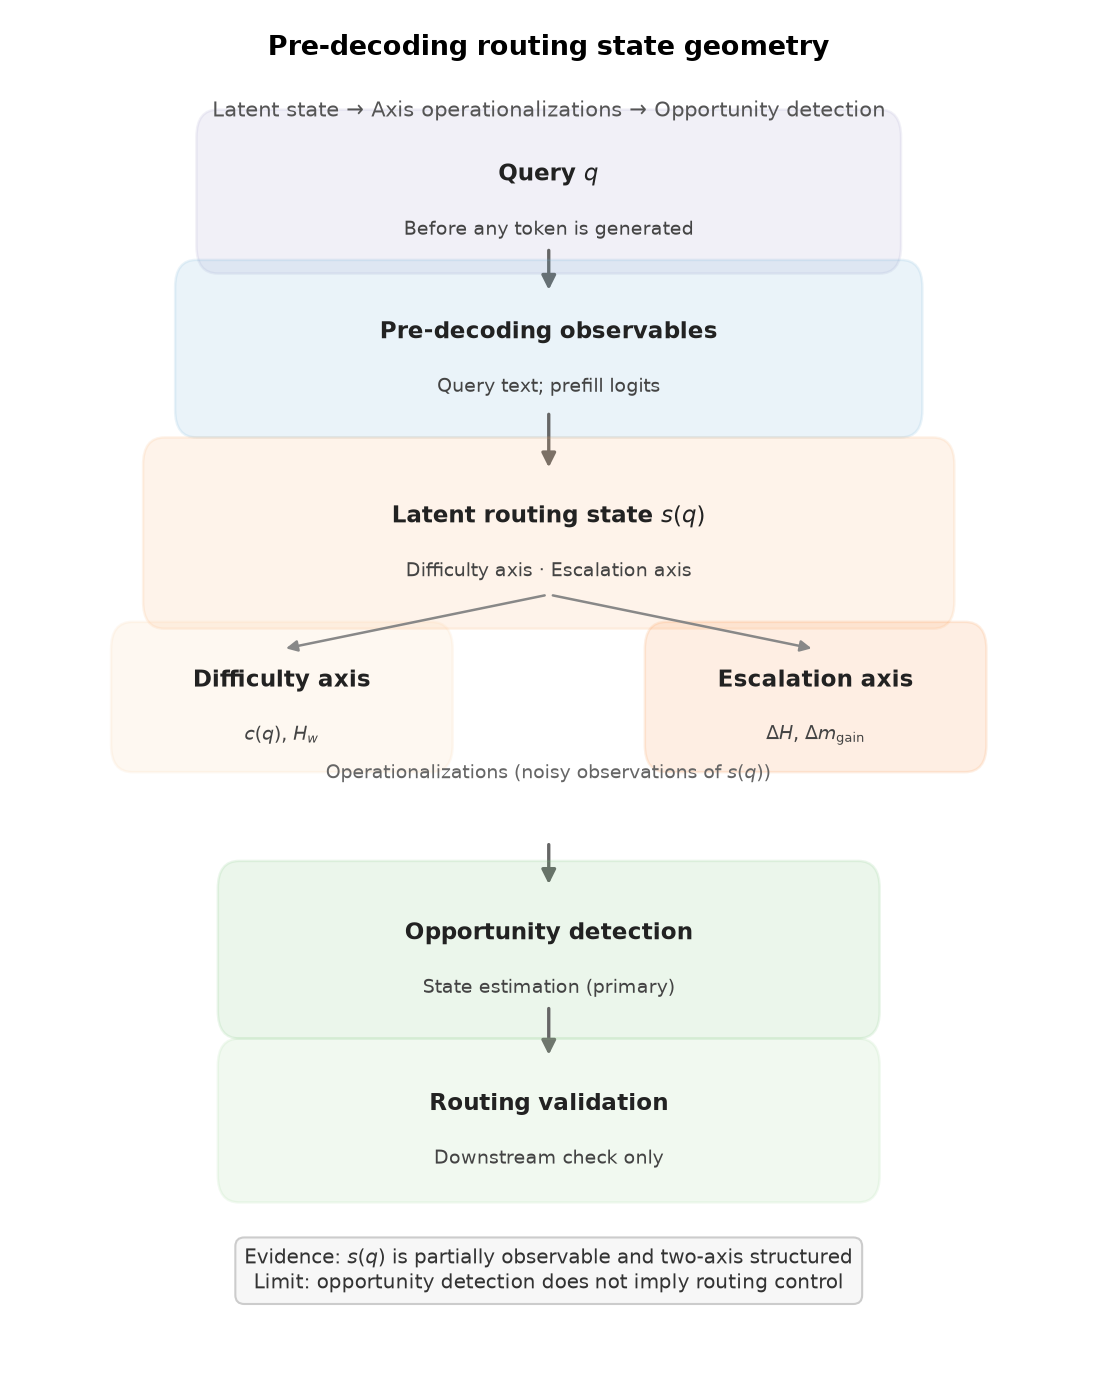
\includegraphics[width=\linewidth]{figures/F0_conceptual_model.png}
  \caption{Unsupervised pre-inference routing via \textbf{latent routing dimensions}. Each dimension is operationalized by a prefill statistic; the scientific unit is the dimension, not the statistic.}
  \label{fig:conceptual}
\end{figure}

\subsection{Finding 1: Latent dimensions predict routing opportunity}
\label{sec:char:finding1}

\paragraph{Oracle landscape.}
Table~\ref{tab:buckets} summarizes offline oracle buckets (\S\ref{sec:setup:oracle}).
Routing opportunity occurs on 43.3\% of test queries---the label each dimension is tested against.

\begin{table}[t]
  \centering
  \small
  \begin{tabular}{lrr}
    \toprule
    \textbf{Bucket} & \textbf{Count} & \textbf{Rate} \\
    \midrule
    Easy & 304 & 25.9\% \\
    Opportunity & 507 & 43.3\% \\
    Weak-only & 61 & 5.2\% \\
    Too-hard & 300 & 25.6\% \\
    \midrule
    \textbf{Total} & \textbf{1{,}172} & \textbf{100\%} \\
    \bottomrule
  \end{tabular}
  \caption{Oracle bucket distribution on ARC test.}
  \label{tab:buckets}
\end{table}

\paragraph{Dimension-wise predictiveness (Studies I--II).}
Table~\ref{tab:study2} reports, for each operationalized dimension, association with $y^{\text{opp}}$.
\textbf{Escalation potential} ($\Delta m_{\mathrm{gain}}$) and \textbf{model disagreement} ($\Delta H$) are the strongest predictors (AUROC ${\sim}0.60$--$0.61$); \textbf{task difficulty} is weaker (AUROC $0.541$).
\textbf{Multiple dimensions carry predictive content}, but none approaches perfect opportunity detection.

% T2: which latent routing dimension predicts opportunity? (ARC TEST)
\begin{table}[t]
  \centering
  \small
  \begin{tabular}{llccc}
    \toprule
    \textbf{Latent routing dimension} & \textbf{Operationalization} & $\rho_s$ [95\% CI] & AUROC [95\% CI] & AUPRC \\
    \midrule
    Task difficulty & $c(q)$ & $+0.071$ [$+0.015$, $+0.128$] & $0.541$ [$0.509$, $0.574$] & $0.474$ \\
    Model uncertainty & $H_w$ & $+0.138$ [$+0.082$, $+0.193$] & $0.581$ [$0.547$, $0.613$] & $0.500$ \\
    Model disagreement & $\Delta H$ & $+0.174$ [$+0.118$, $+0.232$] & $0.602$ [$0.569$, $0.635$] & $0.559$ \\
    Escalation potential & $\Delta m_{\mathrm{gain}}$ & $+0.179$ [$+0.123$, $+0.239$] & $0.605$ [$0.572$, $0.637$] & $0.547$ \\
  \end{tabular}
  \caption{Which \textbf{latent routing dimension} predicts routing opportunity? Predictive association of each operationalized dimension with $y^{\text{opp}}$ on ARC test ($n{=}1{,}172$). AUROC summarizes detectability; the scientific question is dimensional, not a feature leaderboard.}
  \label{tab:study2}
\end{table}


\begin{figure}[t]
  \centering
  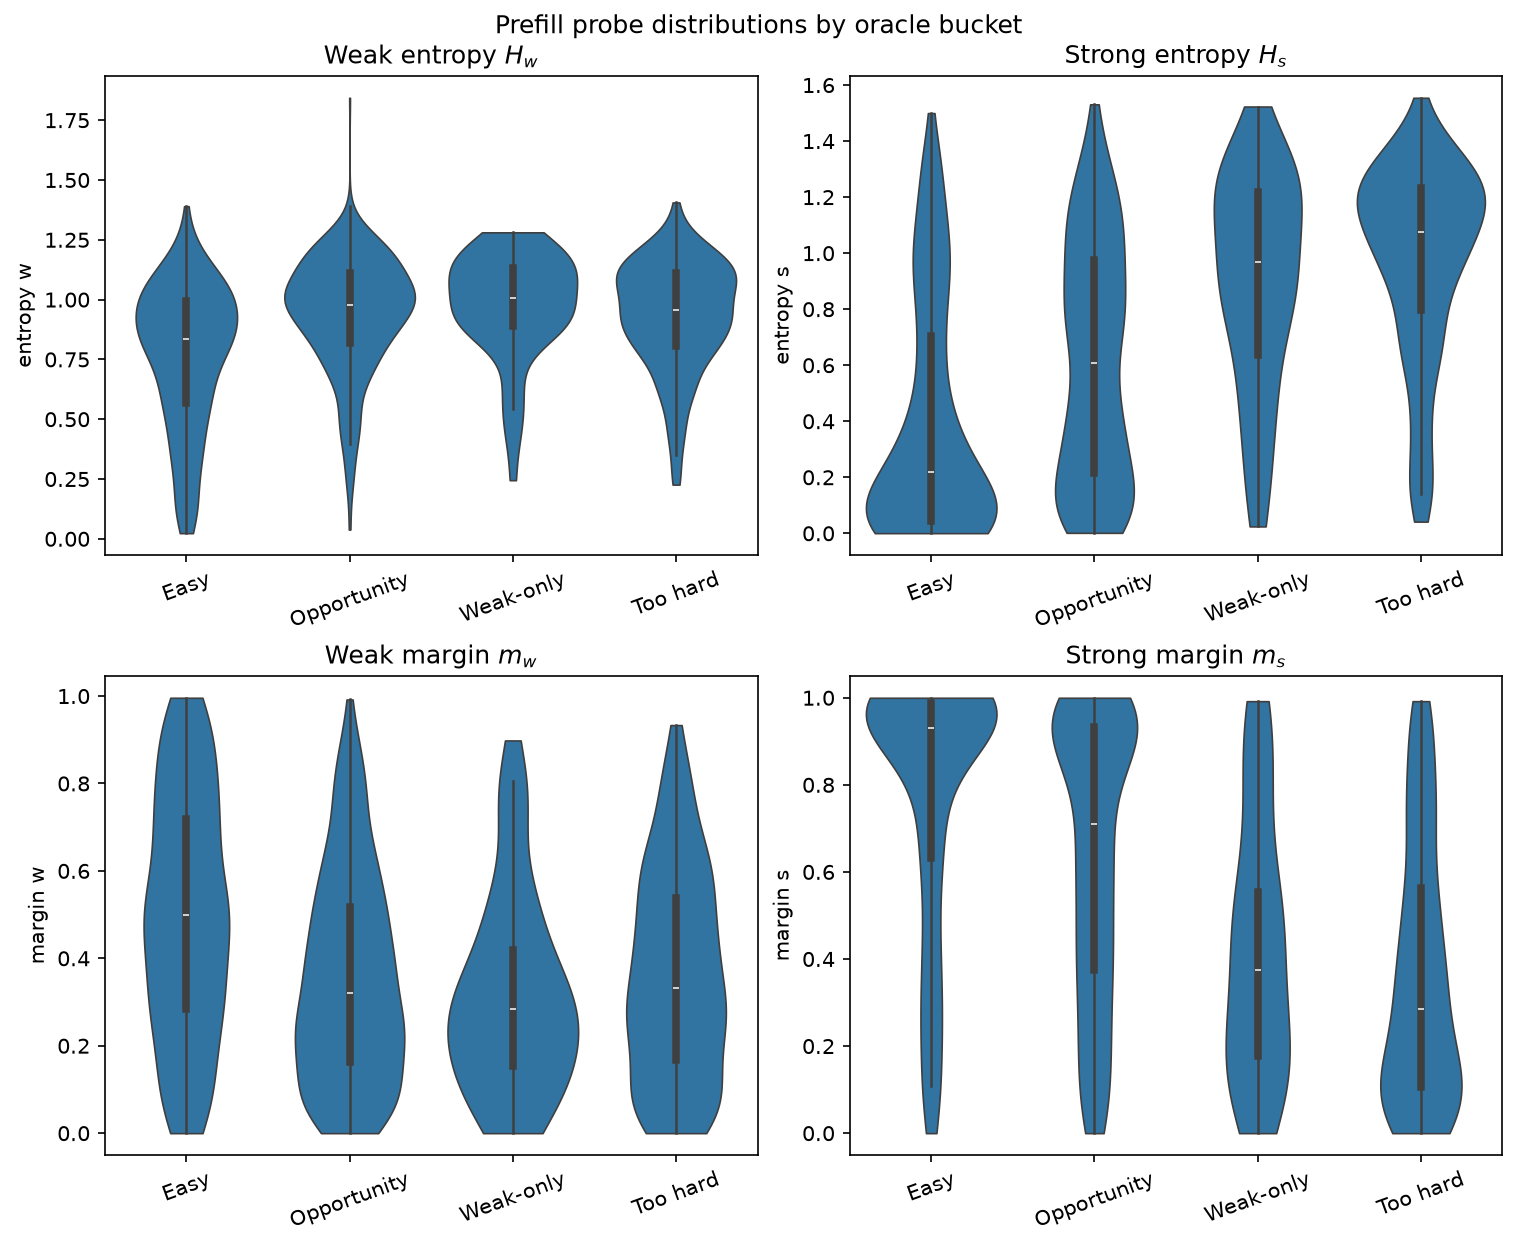
\includegraphics[width=\linewidth]{figures/F1_bucket_distributions.png}
  \caption{Operationalized dimensions by oracle bucket on ARC test.}
  \label{fig:signal-dist}
\end{figure}

\subsection{Finding 2: Dimensions encode different aspects of routing need}
\label{sec:char:finding2}

\paragraph{Cross-dimension structure.}
Dimensions are not interchangeable predictors of the same latent quantity.
Figure~\ref{fig:semantics} contrasts \textbf{model uncertainty} ($H_w$) with \textbf{escalation potential} ($\Delta m_{\mathrm{gain}}$)---both from prefill logits but indexing different routing need.

\begin{figure}[t]
  \centering
  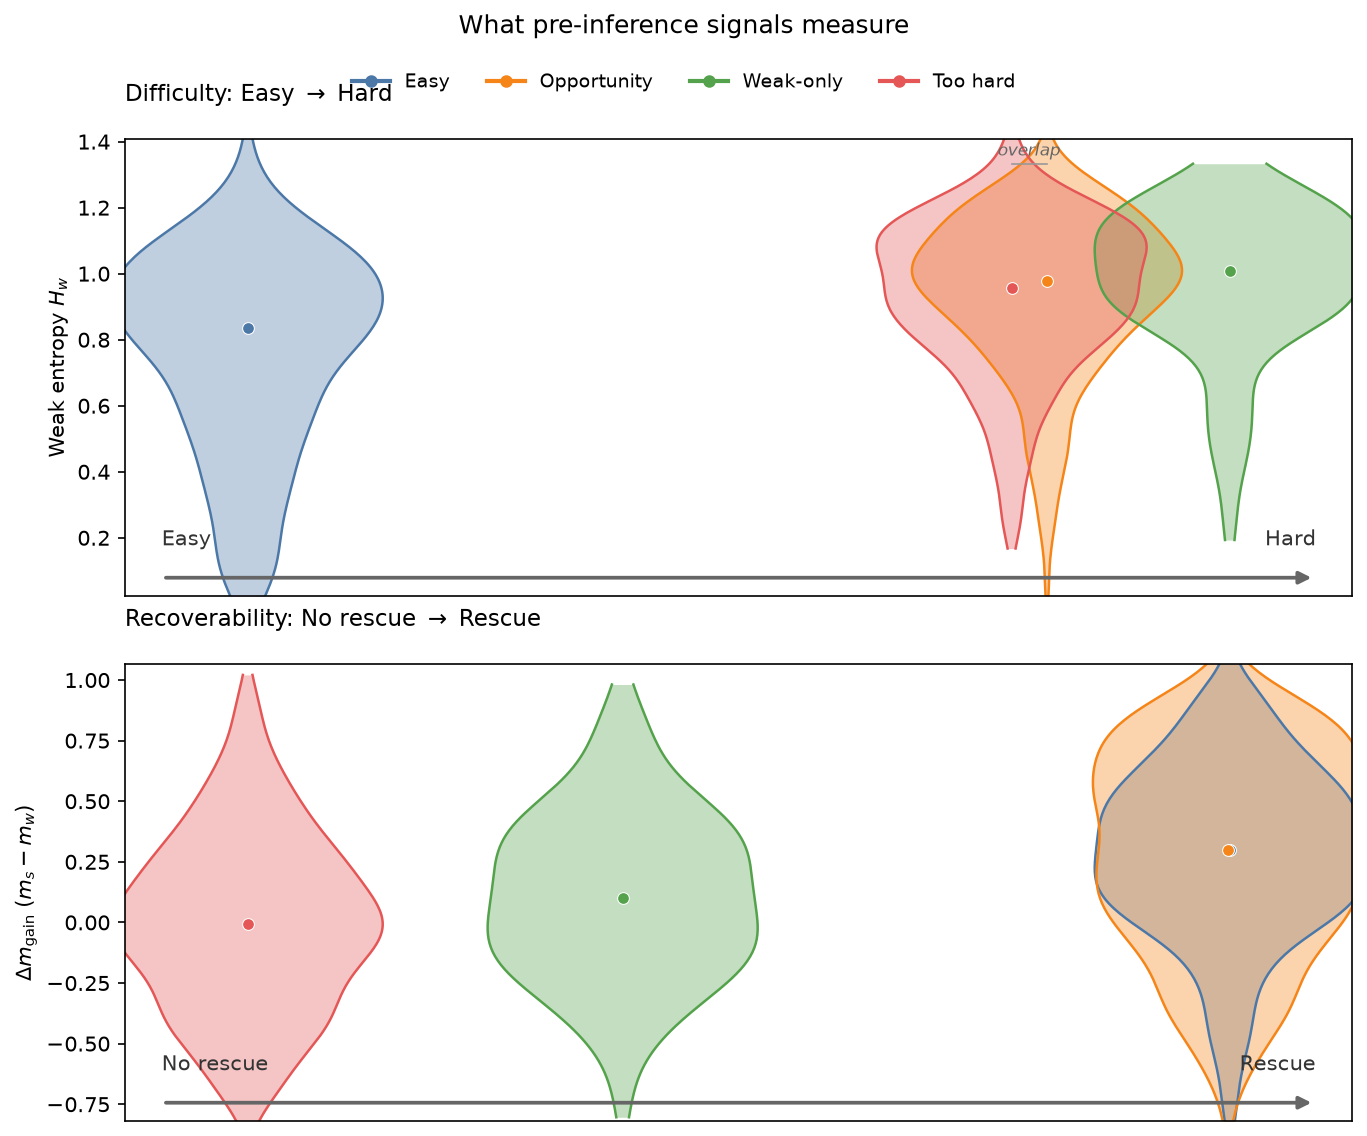
\includegraphics[width=\linewidth]{figures/F2_signal_semantics.png}
  \caption{Model uncertainty vs.\ escalation potential, by oracle bucket.}
  \label{fig:semantics}
\end{figure}

\paragraph{Opportunity vs.\ too-hard.}
Comparing opportunity ($n{=}507$) and too-hard ($n{=}300$):
model uncertainty ($H_w$): $d{\approx}0.03$; escalation potential ($\Delta m_{\mathrm{gain}}$): $d{\approx}0.72$; model disagreement ($\Delta H$): $d{\approx}0.82$.
\textbf{Difficulty-side dimensions} (task difficulty, model uncertainty) do not separate routable from irrecoverable hard queries; \textbf{escalation-side dimensions} (model disagreement, escalation potential) do.

\paragraph{Recovery matrix.}
Figure~\ref{fig:recovery} crosses model uncertainty and escalation potential (median splits).
Highest opportunity rate (57.2\%; $n{=}353$): weak-uncertain queries where the strong model rescues.

\begin{figure}[t]
  \centering
  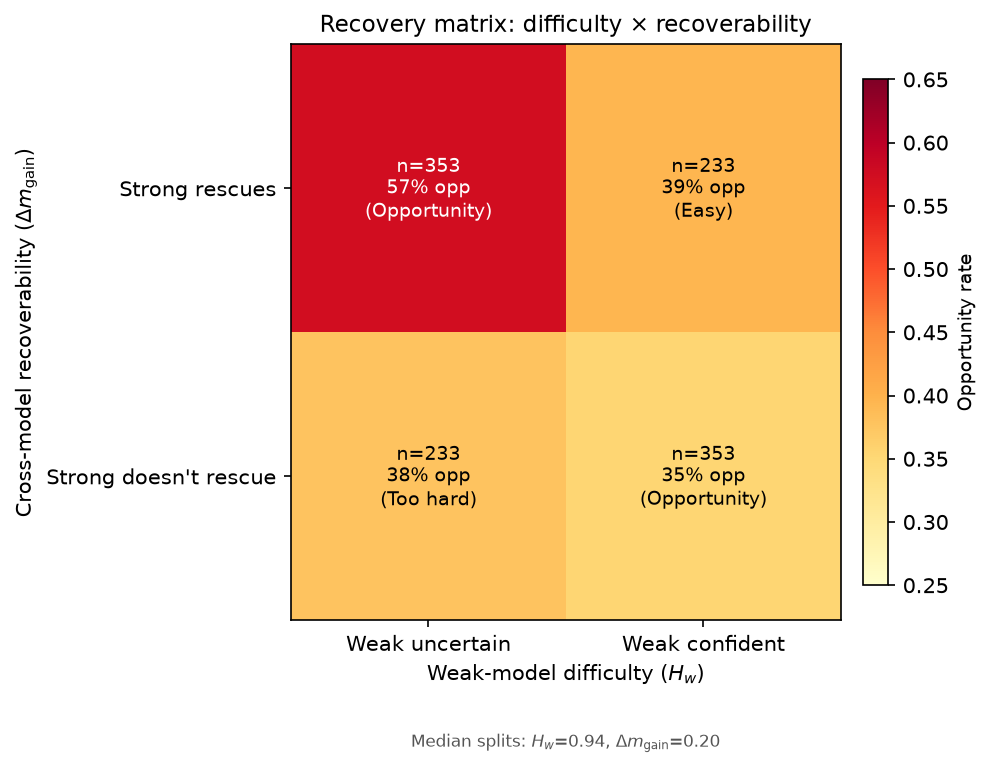
\includegraphics[width=0.92\linewidth]{figures/F6_recovery_matrix.png}
  \caption{Opportunity rate by model uncertainty ($H_w$) and escalation potential ($\Delta m_{\mathrm{gain}}$).}
  \label{fig:recovery}
\end{figure}

\subsection{Complementary predictive content (Study III)}
\label{sec:char:study3}

Adding \textbf{model uncertainty} to \textbf{task difficulty} yields $\Delta$AUROC $= +0.049$ (DeLong $p{=}0.008$): the two dimensions capture partially non-redundant predictive content.
An alternate operationalization of uncertainty ($m_w$) does not improve the joint model on ARC.
Figure~\ref{fig:decomposition} and Table~\ref{tab:complementarity} summarize the dimensional ladder.

% T3: Study III — complementarity ladder (fill after complementarity JSON)
\begin{table}[t]
  \centering
  \small
  \begin{tabular}{lcc}
    \toprule
    \textbf{Model} & \textbf{Features} & AUROC [95\% CI] \\
    \midrule
    Complexity only & $c(q)$ & TBD \\
    Entropy only & $H_w$ & TBD \\
    Margin only & $m_w$ & TBD \\
    $c + H$ & $c, H_w$ & TBD \\
    $c + m$ & $c, m_w$ & TBD \\
    \textbf{Joint (primary)} & $c, H_w, m_w$ & \textbf{TBD} \\
    \midrule
    $\Delta$AUROC ($c \rightarrow c{+}H{+}m$) & --- & \textbf{TBD} \\
    DeLong $p$ & --- & TBD \\
    \bottomrule
  \end{tabular}
  \caption{Study III (RH3): complementary predictive information on ARC test. Primary endpoint: $\Delta$AUROC from $c(q)$ to $c{+}H_w{+}m_w$.}
  \label{tab:complementarity}
\end{table}


\begin{figure}[t]
  \centering
  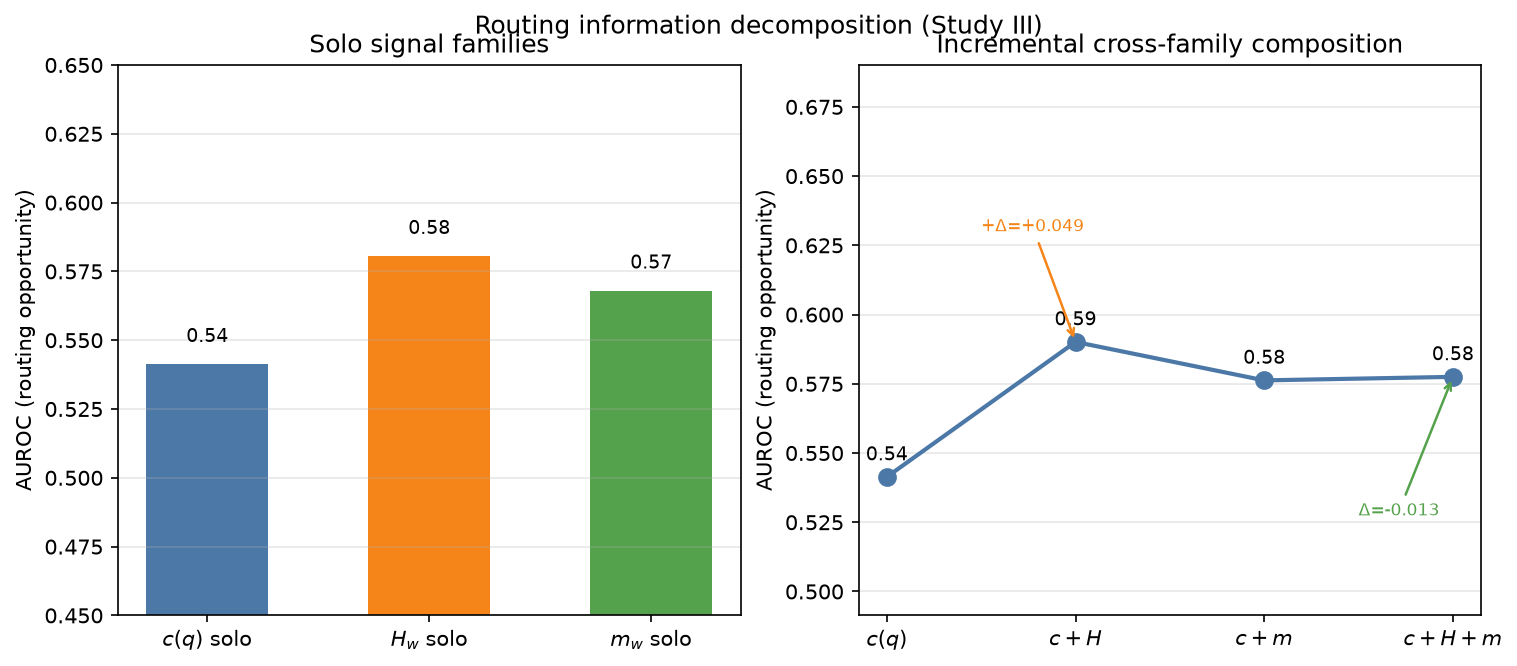
\includegraphics[width=\linewidth]{figures/F3_information_decomposition.png}
  \caption{Complementarity across operationalized dimensions (CALIB-fit, TEST-eval).}
  \label{fig:decomposition}
\end{figure}

\subsection{Probe cost}
\label{sec:char:cost}

Table~\ref{tab:probe-cost} compares prefill-probe cost to post-generation routing \citep{guha2024smoothie,kotte2026ucci,hu2024routerbench}.

\begin{table}[t]
  \centering
  \small
  \begin{tabular}{ll}
    \toprule
    \textbf{Strategy} & \textbf{Relative cost} ($m{=}2$) \\
    \midrule
    Always weak & 1 generation \\
    Always strong & 3 generations \\
    Prefill probes & $\ll 1$ generation \\
    Post-generation routing & 2 generations \\
    \bottomrule
  \end{tabular}
  \caption{Prefill probes vs.\ full generation cost.}
  \label{tab:probe-cost}
\end{figure}


\section{Routing Evaluation}
\label{sec:routing}
% §6 Routing evaluation (Study IV)

Study~IV performs \textbf{routing evaluation}: given the evidence in \S\ref{sec:characterization}, can pre-inference signals support appropriate model selection?
We use a calibrated logistic policy as an evaluation instrument---not a routing contribution \citep{cao2026scope}.

\subsection{Routing policy}
\label{sec:routing:policy}

Fit on CALIB: $\hat{p}(q) = P(y^{\text{opp}}{=}1 \mid c, H_w, m_w)$; tune $\tau$ for $U = \text{accuracy} - \lambda \cdot \text{cost}$; evaluate on TEST.
Assign $M_s$ if $\hat{p}(q) \geq \tau$; else $M_w$.

\subsection{Baselines}
\label{sec:routing:baselines}

Always-weak, always-strong, calibrated logistic policy, offline oracle \citep{hu2024routerbench}.
Cost: weak $=1$, strong $=3$.

\subsection{Finding 3: Routing leaves exploitable headroom}
\label{sec:routing:results}

% T4: Study IV — decision utility (fill after route-eval JSON; run per cost_lambda)
\begin{table}[t]
  \centering
  \small
  \begin{tabular}{lccccc}
    \toprule
    \textbf{Policy} & $\boldsymbol{\lambda}$ & \textbf{Acc.} & \textbf{Avg.\ cost} & $\boldsymbol{U}$ & \textbf{Opp.\ recall} \\
    \midrule
    Always-weak    & --- & TBD & TBD & TBD & TBD \\
    Always-strong  & --- & TBD & TBD & TBD & TBD \\
    Learned router & 0    & TBD & TBD & TBD & TBD \\
    Learned router & 0.05 & TBD & TBD & TBD & TBD \\
    Learned router & 0.10 & TBD & TBD & TBD & TBD \\
    Oracle (bound) & --- & TBD & TBD & --- & 100\% \\
    \bottomrule
  \end{tabular}
  \caption{Study IV (RH4): decision utility on ARC test. Router fit on CALIB; $\tau$ tuned per $\lambda$; $U=\text{acc}-\lambda\cdot\text{cost}$.}
  \label{tab:routing}
\end{table}


At $\lambda{=}0$, the calibrated policy matches always-strong (69.2\%).
The oracle reaches 74.4\%: \textbf{5.2 percentage points} of headroom, \textbf{none} exploited ($\tau{=}0$).

\paragraph{Interpretation.}
Before generation, there is useful---but incomplete---information for selecting the appropriate LLM.
Finding~2 explains part of the gap: policies that conflate \textbf{model uncertainty} with \textbf{escalation potential} cannot select appropriately.
Detection (${\sim}0.61$ AUROC) exceeds assignment under this policy class \citep{plaut2024chat,hu2024routerbench}.


\section{Discussion}
\label{sec:discussion}
% §7 Discussion

\subsection{Synthesis}
\label{sec:disc:synthesis}

We asked whether unsupervised pre-inference signals can support appropriate multi-LLM routing before generation.
On ARC-Challenge, the answer is \textbf{partially}.

The scientific contribution is dimensional: routing need decomposes into \textbf{latent dimensions}---task difficulty, model uncertainty, model disagreement, escalation potential---each operationalized by a prefill statistic.
Before generation, multiple dimensions predict routing opportunity; they encode \textbf{different aspects of routing need}.
A calibrated routing policy does not fully exploit what is available.

\subsection{Why the dimensional view matters}
\label{sec:disc:failures}

Treating \textbf{model uncertainty} as a proxy for \textbf{escalation potential} fails: opportunity and too-hard queries are indistinguishable on $H_w$ yet separate on $\Delta m_{\mathrm{gain}}$.
Routing policies must respect the dimensional structure documented in \S\ref{sec:char:finding2}.

\subsection{Future dimensions}
\label{sec:disc:future}

This study operationalizes four dimensions from query text and single-step prefill logits.
Richer measurements---generation trajectories, hidden states, paraphrase stability---may support additional latent dimensions (appendix Table~\ref{tab:dim-taxonomy}) without changing the dimensional abstraction.

\subsection{Limitations}
\label{sec:disc:limits}

Binary Llama~3.2 pool; ARC-Challenge only; one operationalization per main dimension; demonstration policy calibrated on CALIB.


\section{Conclusion}
\label{sec:conclusion}
% §8 Conclusion

We studied whether unsupervised pre-inference signals can support appropriate multi-LLM routing before generation.
We framed routing need as \textbf{latent dimensions}---task difficulty, model uncertainty, model disagreement, escalation potential---each operationalized by a prefill statistic, and asked which dimensions predict routing opportunity on ARC-Challenge.

\textbf{Multiple dimensions predict opportunity} (best AUROC ${\sim}0.61$ for escalation potential).
\textbf{Dimensions differ}: difficulty-side and escalation-side operationalizations separate different routing need.
\textbf{Routing leaves headroom}: 5.2 percentage points above always-strong remain unexploited by a calibrated policy.

The contribution is a dimensional map of pre-inference routing information---not a feature correlation study and not a new supervised router.


\bibliographystyle{plainnat}
\bibliography{references}

\appendix
% Appendix sections (included from acl.tex after \appendix)

\section{Configuration screening}
\label{app:validation}

Before locking the primary $(\text{pool}, \text{dataset}, \text{prompt formatting})$ triple, we screened candidates on small samples ($n{=}5$--$10$, seed 42) for non-degenerate routing opportunity and successful prefill extraction (\S\ref{sec:setup:config}).
Table~\ref{tab:config-screen} summarizes pilot outcomes.
Qwen~2.5~1.5B/3B on GSM8K ($n{=}5$) yielded 100\% too-hard buckets (both models failed all items).
The same Qwen pool on ARC ($n{=}10$) yielded 0\% opportunity with 70\% easy---weak model already succeeds on most items.
Llama~3.2~1B/3B on ARC showed 50\% opportunity on $n{=}10$ and ${\sim}24\%$ on a ${\sim}50$-query pilot, motivating the locked configuration reported in the main text ($n{=}1{,}172$ test; 43.3\% opportunity).

% Appendix: configuration screening (pilot samples; not reported metrics)
\begin{table}[t]
  \centering
  \small
  \begin{tabular}{llrrl}
    \toprule
    \textbf{Pool} & \textbf{Dataset} & $n$ & Opp.\ \% & \textbf{Outcome} \\
    \midrule
    Qwen 1.5B / 3B & GSM8K test & 5 & 0\% & Excluded: 100\% too-hard \\
    Qwen 1.5B / 3B & ARC-Challenge & 10 & 0\% & Excluded: 70\% easy \\
    Llama 1B / 3B & ARC-Challenge & 10 & 50\% & Studiable (pilot) \\
    Llama 1B / 3B & ARC-Challenge & ${\sim}50$ & ${\sim}24$\% & Non-degenerate mix \\
    \textbf{Llama 1B / 3B} & \textbf{ARC-Challenge} & \textbf{1{,}172} & \textbf{43.3\%} & \textbf{Locked (TEST)} \\
    \bottomrule
  \end{tabular}
  \caption{Requirements-first configuration search (seed 42). Pilot runs select a studiable $(\text{pool}, \text{dataset})$ triple; only the locked row contributes paper metrics.}
  \label{tab:config-screen}
\end{table}


\section{Complexity dimension candidate screening}
\label{app:d46}

Representative $c(q)$ is selected once on CALIB before test evaluation (\S\ref{sec:setup:calib}).
Table~\ref{tab:d46} reports all five tokenizer-based candidates scored against $y^{\text{opp}}$ on ARC validation ($n{=}299$).
\texttt{piece\_count} wins by the frozen composite rule despite modest absolute $\rho$ and AUROC; compressibility and normalized Shannon entropy rank higher on $|\rho|$ alone but lower on AUROC.
We report partial correlation $\rho(c,y^{\text{opp}}\mid\text{length})=-0.448$ on CALIB as a length-confound diagnostic for the selected feature.

% Appendix: D46 model-independent candidate screening (ARC CALIB, n=299)
\begin{table}[t]
  \centering
  \small
  \begin{tabular}{llccc}
    \toprule
    \textbf{Family} & \textbf{Candidate} & $\rho_s$ [95\% CI] & AUROC [95\% CI] & Composite \\
    \midrule
    Length & \texttt{piece\_count} & $+0.093$ [$-0.024$, $+0.210$] & $0.556$ [$0.486$, $0.629$] & 4.0 \\
    Lexical diversity & \texttt{mattr} & $-0.067$ [$-0.179$, $+0.048$] & $0.460$ [$0.395$, $0.530$] & 2.5 \\
    Information & \texttt{text\_shannon} & $-0.015$ [$-0.121$, $+0.099$] & $0.491$ [$0.426$, $0.560$] & 2.5 \\
    Information & \texttt{text\_shannon\_norm} & $-0.151$ [$-0.264$, $-0.039$] & $0.409$ [$0.345$, $0.481$] & 3.0 \\
    Compressibility & \texttt{compression\_ratio} & $-0.172$ [$-0.282$, $-0.061$] & $0.397$ [$0.328$, $0.465$] & 3.0 \\
    \bottomrule
  \end{tabular}
  \caption{D46 screening on ARC validation (CALIB, $n{=}299$). Selection maximizes composite $\tfrac{1}{2}\mathrm{rank}(|\rho|)+\tfrac{1}{2}\mathrm{rank}(\mathrm{AUROC})$; winner \texttt{piece\_count} frozen as $c(q)$ for all test reporting. Partial $\rho(c,y^{\text{opp}}\mid\text{length})=-0.448$ on CALIB (length confound diagnostic).}
  \label{tab:d46}
\end{table}


\section{Model-dependent probe variants}
\label{app:md-variants}

Prefill extraction logs auxiliary statistics from the same forward pass (\S\ref{sec:method:prefill}).
Table~\ref{tab:md-variants} audits redundancy on ARC test.
Normalized entropy, top-10 entropy, and effective vocabulary size $n_{\mathrm{eff}}=\exp(H_w)$ are numerically redundant with full-vocabulary $H_w$ ($\rho_s{\approx}1.0$; AUROC within 0.001).
Among derived cross-model statistics, $\Delta n_{\mathrm{eff}}$ achieves the highest opportunity AUROC (0.616) but does not change the recoverability interpretation relative to $\Delta m_{\mathrm{gain}}$ and $\Delta H$.

% Appendix: model-dependent probe variant redundancy (ARC TEST, n=1172)
\begin{table}[t]
  \centering
  \small
  \begin{tabular}{lccr}
    \toprule
    \textbf{Signal} & $\rho_s(H_w,\cdot)$ & Opp.\ AUROC & \textbf{Note} \\
    \midrule
    \multicolumn{4}{l}{\textit{Weak prefill variants}} \\
    $H_w$ (full vocab) & 1.000 & 0.581 & headline \\
    $H_{\mathrm{norm}}$ & 1.000 & 0.581 & redundant \\
    $H_{\mathrm{top10}}$ & 0.9998 & 0.580 & redundant \\
    $n_{\mathrm{eff}}$ & 1.000 & 0.581 & redundant ($e^{H_w}$) \\
    $m_w$ & $-0.819$ & 0.568$^\dagger$ & direction flipped \\
    $p_{\max}$ & $-0.911$ & 0.574$^\dagger$ & correlated with $H_w$ \\
  \addlinespace
    \multicolumn{4}{l}{\textit{Cross-model derived}} \\
    $\Delta H$ & --- & 0.602 & headline \\
    $\Delta H_{\mathrm{norm}}$ & --- & 0.601 & redundant \\
    $\Delta H_{\mathrm{top10}}$ & --- & 0.601 & redundant \\
    $\Delta n_{\mathrm{eff}}$ & --- & 0.616 & best single AUROC \\
    $\Delta m_{\mathrm{gain}}$ & --- & 0.605 & recoverability rep. \\
    \bottomrule
  \end{tabular}
  \caption{Probe variant audit on ARC test. $^\dagger$AUROC after sign flip (higher score $\Rightarrow$ higher opportunity). Variants logged at extraction time; main text uses $H_w$, $m_w$, $\Delta H$, $\Delta m_{\mathrm{gain}}$ only.}
  \label{tab:md-variants}
\end{table}


\section{Information dimension taxonomy (extended)}
\label{app:dimensions}

Table~\ref{tab:dim-taxonomy} lists candidate statistics for each information dimension.
The main analysis reports bold representatives only; additional rows indicate future measurements without expanding headline claims.

% Extended dimension taxonomy (candidates; not main-paper claims). Bold rows match Table~\ref{tab:dimensions}.
\begin{table}[t]
  \centering
  \footnotesize
  \setlength{\tabcolsep}{3pt}
  \begin{tabular}{@{}p{0.14\linewidth}p{0.20\linewidth}p{0.58\linewidth}@{}}
    \toprule
    \textbf{Dimension} & \textbf{Source} & \textbf{Candidate statistics; main study in bold} \\
    \midrule
    \textbf{Complexity} & Query text &
    \textbf{\texttt{piece\_count}}, MATTR, MTLD, compression, text Shannon, sentence count, choice count, prompt length \\
    \addlinespace
    \textbf{Uncertainty} & $M_i$ logits &
    \textbf{$H$}, $H_{\mathrm{top10}}$, $n_{\mathrm{eff}}$, tail entropy, R\'enyi \\
    \addlinespace
    Confidence & $M_i$ logits &
    \textbf{$m$}, $p_{\max}$, top-5 mass, log-odds \\
    \addlinespace
    \textbf{Agreement} & $M_w{\leftrightarrow}M_s$ &
    \textbf{$\Delta H$}, KL, JS divergence, rank correlation \\
    \addlinespace
    \textbf{Recoverability} & $M_w{\leftrightarrow}M_s$ &
    \textbf{$\Delta m_{\mathrm{gain}}$}, $\Delta p_{\max}$, $\Delta n_{\mathrm{eff}}$ \\
    \addlinespace
    Dynamics & Generation trajectory &
    entropy slope, margin slope, trajectory variance (future work) \\
    \addlinespace
    Representation & Hidden states &
    layer norms, hidden similarity (future work) \\
    \addlinespace
    Stability & Paraphrase / multi-probe &
    cross-paraphrase variance (deferred) \\
    \addlinespace
    Calibration & Offline fit &
    ECE, temperature, Brier (deferred) \\
    \bottomrule
  \end{tabular}
  \caption{Extended information-dimension taxonomy. Main text reports bold representatives only; additional rows indicate future measurements without expanding headline claims.}
  \label{tab:dim-taxonomy}
\end{table}


\section{Calibration diagnostics}
\label{app:calibration}

Figure~\ref{fig:entropy-calib} shows weak entropy $H_w$ quantile calibration against opportunity rate on TEST (decile bins).
Figure~\ref{fig:prob-calib} shows probability calibration of the joint logistic model from Study~IV (CALIB-fit, TEST-eval).
The joint model is underconfident (mean signed gap $-0.037$ per bin), consistent with degenerate routing $\tau{=}0$ on TEST (\S\ref{sec:routing:results}).

\begin{figure}[t]
  \centering
  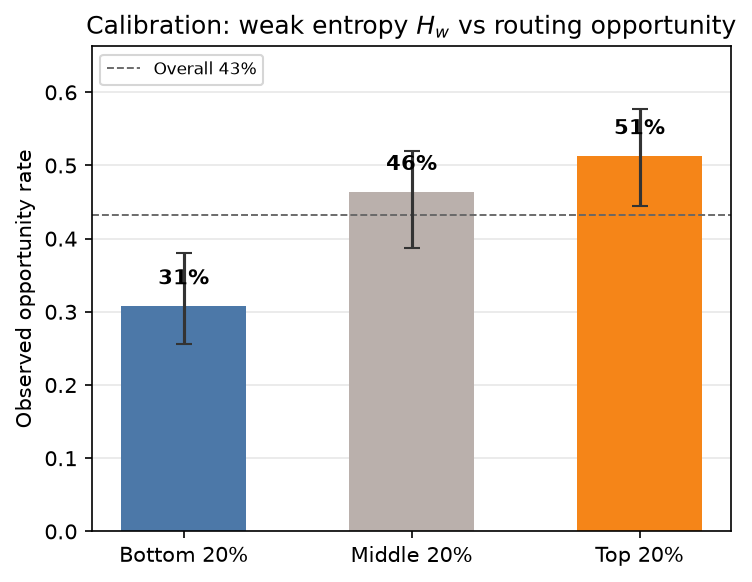
\includegraphics[width=0.92\linewidth]{figures/F4_entropy_calibration.png}
  \caption{Weak entropy $H_w$ quantile calibration vs.\ observed opportunity rate (ARC test).}
  \label{fig:entropy-calib}
\end{figure}

\begin{figure}[t]
  \centering
  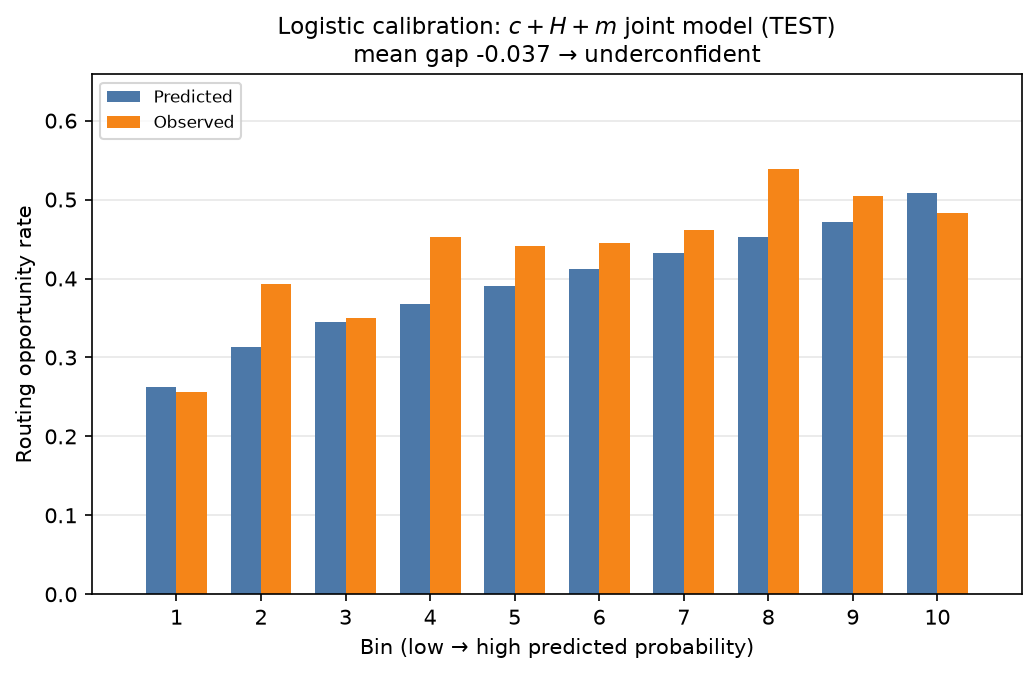
\includegraphics[width=0.92\linewidth]{figures/F5_probability_calibration.png}
  \caption{Joint logistic $\Pr(y^{\text{opp}}\mid c,H_w,m_w)$ calibration (CALIB-fit, TEST-eval).}
  \label{fig:prob-calib}
\end{figure}


\end{document}
